\documentclass[11pt]{article}
\textwidth 15.9cm
\textheight 23. cm
\addtolength{\oddsidemargin}{-11.5mm}
\addtolength{\evensidemargin}{-11.5mm}
\addtolength{\topmargin}{-19.0mm}

%\usepackage{amsmath}
\usepackage[ansinew]{inputenc}
\usepackage[bbgreekl]{mathbbol}
\usepackage{amsmath,amssymb}
\usepackage{graphicx}
\usepackage{hyperref}
\usepackage{url}
\usepackage[numbers,square]{natbib}
\usepackage{multirow}
\usepackage{tikz}
\usepackage{tikz-cd}
\usetikzlibrary{arrows,matrix}
\usepackage{bbm}
\usepackage{authblk}
\usepackage{subcaption}
\renewcommand{\Affilfont}{\footnotesize}
%\renewcommand{\Authfont}{\normalsize}

\usepackage{stmaryrd}
\usepackage{comment}
\usepackage{showlabels}
\usepackage{soul}
%\usepackage[dvipsnames]{xcolor}

\usetikzlibrary{calc,patterns,shapes.geometric}
\usetikzlibrary{arrows,shapes,positioning}
\usetikzlibrary{decorations.markings,decorations.pathmorphing,decorations.pathreplacing}
\usetikzlibrary{decorations.text,decorations.shapes}

%%%%%%%% MACROS
\include{gempic_spectral_macros}

\newcommand{\hi}{\hat{i}}
\newcommand{\hj}{\hat{j}}
\newcommand{\hk}{\hat{k}}

% \newcommand{\arr}[1]{{\bs{\mathsf{#1}}}}

% matrices
\newcommand{\hodgeZero}{\mathbb{H}_0}
\newcommand{\hodgeOne}{\mathbb{H}_1}
\newcommand{\hodgeTwo}{\mathbb{H}_2}
\newcommand{\hodgeThree}{\mathbb{H}_3}
\newcommand{\hodgeDualZero}{\tilde{\mathbb{H}}_0}
\newcommand{\hodgeDualOne}{\tilde{\mathbb{H}}_1}
\newcommand{\hodgeDualTwo}{\tilde{\mathbb{H}}_2}
\newcommand{\hodgeDualThree}{\tilde{\mathbb{H}}_3}
\newcommand{\hodgeDualZeroB}{\mathbb{H}^*_0}
\newcommand{\hodgeDualOneB}{\mathbb{H}^*_1}
\newcommand{\hodgeDualTwoB}{\mathbb{H}^*_2}
\newcommand{\hodgeDualThreeB}{\mathbb{H}^*_3}

\newtheorem{theorem}{Theorem}
\newtheorem{lemma}{Lemma}
\newtheorem{remark}{Remark}
\newtheorem{definition}{Definition}
\newtheorem{assumption}{Assumption}



\title{Notation conventions in GEMPIC}


\author[1]{The Gempic development team}
\affil[1]{Max-Planck-Institut f\"ur Plasmaphysik, Garching, Germany}



\begin{document}



\maketitle

\begin{abstract}
This note describes some conventions that should be followed in the GEMPIC code
and its documentation.
\end{abstract}

\tableofcontents

\section{Notation for de Rham diagrams }


The structure-preserving methods used in GEMPIC schemes rely on two de Rham sequences, one primal and another one dual. 
At the continuous level this is symmetric, and one usually consists of differential operators which are the adjoints of the other one:
see e.g. \cite[Sec.~3]{Arnold.Falk.Winther.2010.bams} 
for a description in terms of Hilbert complexes.

\subsection{General notation for primal-dual de Rham diagrams}

At the discrete level the general case is represented by the following diagram:

\begin{equation}
	\label{CGL}
	~
\end{equation}

\begin{figure}
	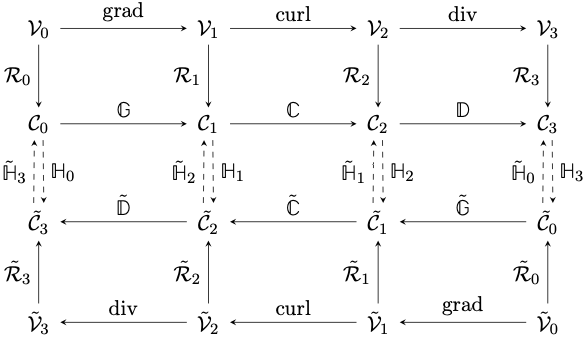
\includegraphics[width=130mm]{deRhamCGL.png}
\end{figure}


A few observations are in order.
\begin{itemize}
    \item This notation preserves the symmetry:
		in both complexes the discrete differential operators correspond to the strong operators of their continuous sequence, and the space numbers are intrinsic as they correspond to the degree of the differential forms.
		
		\item The Hodge operators are written with only one index corresponding to the starting space (and $\tilde{\mathbb{H}}$ if it starts from the dual complex).

		\item The diagrams should commute except for the dashed lines (i.e. the Hodge operators). In particular, the dual Hodge operators do not need to be inverse of the primal ones
		(they do not even need to be represented by square matrices).

		\item Here the spaces $\cV_\ell$ and $\tilde{\cV}_\ell$ in the continuous sequences 
		are a priori infinite-dimensional function spaces. A standard choice corresponding
		to the Hilbert-complex theoretical framework of \cite{Arnold.Falk.Winther.2010.bams}
		is to take $L^2$ spaces with $L^2$ derivatives and proper boundary conditions as 
		described below.		
		
		\item The reduction (commuting) operators 
		$\cR_\ell$ and $\tilde {\cR}_\ell$ may not be defined 
		on the full spaces $\cV_\ell$ and $\tilde{\cV}_\ell$: their domain spaces may 
		(and often do) consist of smaller spaces of smoother functions.

\end{itemize}

\subsection{Boundary conditions}
\label{sec:bc}

In the full space $\Omega = \RR^3$ or with periodic boundary conditions,
the simplest choice is to consider 
\begin{equation} \label{dR_spaces_nobound}
  \cV_0 = \tilde{\cV}_0 = H^1(\Omega), \quad
    \cV_1 = \tilde{\cV}_1 = H(\curl;\Omega), \quad
      \cV_2 = \tilde{\cV}_2 = H(\Div;\Omega), \quad
        \cV_3 = \tilde{\cV}_3 = L^2(\Omega).
\end{equation}		
In a bounded domain, boundary conditions are in general imposed
so that integration by parts hold between primal and dual spaces without boundary terms,
in the sense that
$$
\sprod{\grad \vp}{\tilde \bC} = -\sprod{\vp}{\Div \tilde \bC},
\qquad
\sprod{\curl \bF}{\tilde \bG} = \sprod{\bF}{\curl \tilde \bG},
\qquad
\sprod{\Div \bC}{\tilde \vp} = -\sprod{\bC}{\grad \tilde \vp}
$$
(with $L^2(\Omega)$ scalar products) 
should hold for all $\vp \in \cV_0$, $\bF \in \cV_1$, $\bC \in \cV_2$,
and all $\tilde \vp \in \tilde{\cV}_0$, $\tilde \bF \in \tilde{\cV}_1$,
$\tilde \bC \in \tilde{\cV}_2$.
For instance if the primal space has no boundary condition,
\begin{equation} \label{dR_spaces_inhom}
	\cV_0 = H^1(\Omega), \quad
    \cV_1 = H(\curl;\Omega), \quad
      \cV_2 = H(\Div;\Omega), \quad
        \cV_3 = L^2(\Omega).
\end{equation}		
then the dual one should have homogeneous conditions
\begin{equation} \label{dR_spaces_hom}
	\tilde{\cV}_0 = H^1_0(\Omega), \quad
    \tilde{\cV}_1 = H_0(\curl;\Omega), \quad
      \tilde{\cV}_2 = H_0(\Div;\Omega), \quad
        \tilde{\cV}_3 = L^2(\Omega).
\end{equation}		
By symmetry, the opposite choice is also valid.


\subsection{Alternate notation for subordinated dual complexes}

In many cases (e.g. standard finite elements or finite differences on staggered grids), the discrete dual complex is completely determined from the primal one and in particular the dual differential operators are represented my matrices which satisfy
\begin{equation} \label{diff_T}
	\tilde{\mathbb{G}} = -\mathbb{D}^\top
	\qquad 
	\tilde{\mathbb{C}} = \mathbb{C}^\top
	\qquad
	\tilde{\mathbb{D}} = -\mathbb{G}^\top
\end{equation}
which implies that the dual discrete spaces $\tilde{\mathcal{C}}_\ell$ have the same dimension as $\mathcal{C}_{3-\ell}$
(for all $\ell$). 
(In finite elements this follows from the fact that the dual discrete spaces coincide with the 
primal ones, $\tilde{V}_\ell = V_{3-\ell}$, and that the dual differentials are defined by discrete duality.)

In this case {\em a natural notation is to label the dual spaces with the indices of their primal counterparts}.
Accordingly the dual differential operators are defined (or seen) as the adjoints of the primal ones.

This results in the following diagram.

\begin{equation}
	\label{CGL2}
	~
\end{equation}

\begin{figure}[h]
	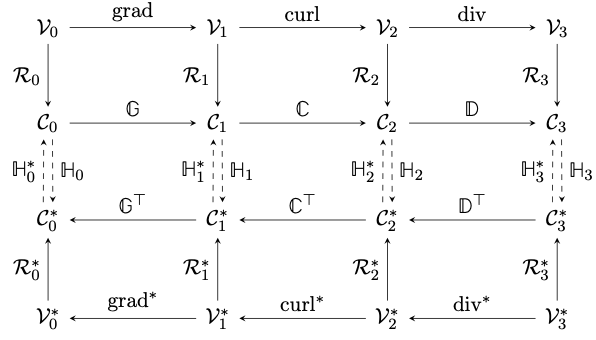
\includegraphics[width=150mm]{deRhamCGL2.png}
\end{figure}	



Here the dual differential operators at the continuous level 
are {\em explicitely defined} as the adjoints of the primal ones,
and the spaces $\cV^*_\ell$ as their {\em domain spaces},
see e.g. \cite[Section~2.6]{Brezis.2011.fa}.
With the choices described in Section~\ref{sec:bc} this yields
\begin{equation} \label{diffadj}
{\grad}^* = -\Div : \cV_3^* \to \cV_2^*
\qquad 
{\curl}^* = \curl : \cV_2^* \to \cV_1^*
\qquad
{\Div}^* = -\grad : \cV_1^* \to \cV_0^*
\end{equation}
with domain spaces given by 
\begin{equation} \label{cV*}
	\cV_\ell^* = \tilde{\cV}_{3-\ell}.
\end{equation}

In particular, this diagram is just another representation of the general diagram \eqref{CGL} 
(if it holds, i.e. if the dual sequence is subordinated to the primal one),
using the relations~\eqref{diffadj}--\eqref{cV*} for the continuous differential operators
and \eqref{diff_T} for the discrete ones. The discrete spaces and reduction resp. Hodge 
operators then coincide,
\begin{equation}
\tilde{\mathcal{C}_\ell} = \mathcal{C}_{3-\ell}^*
\qquad 
\tilde{\mathcal{R}_\ell} = \mathcal{R}_{3-\ell}^*
\qquad 
\tilde{\mathbb{H}_\ell} = \mathbb{H}_{3-\ell}^*
\end{equation}
	

\subsection{Illustration with Maxwell's equations}
We may illustrate these notations with Maxwell's equations 
\begin{equation} \label{max_cont}
	\left\{\begin{aligned}
		&\partial_t {\bs D} - \curl {\bs H} = -{\bs J}
		\\
		&\partial_t {\bs B} + \curl {\bs E} = 0
	\end{aligned}\right.
	\quad \text{with constitutive relations} \quad
	\left\{\begin{aligned}
		&{\bs H} = -\cH_\mu {\bs B}
		\\
		&{\bs D} = -\cH_\ve {\bs D}.
	\end{aligned}\right.	
\end{equation}
Here $\cH_\mu$ and $\cH_\ve$ are continuous Hodge operators
associated with the magnetic and electric permittivity tensors.
For constant permittivities in $\RR^3$ these are simply (scaled) identity operators.
A space discretization using the general diagram \eqref{CGL} is 
\begin{equation} \label{max}
	\left\{\begin{aligned}
		&\partial_t \tilde {\arr{D}} - \tilde{\mathbb{C}} \tilde {\arr{H}} = -\tilde{\arr{J}}
		\\
		&\partial_t \arr{B} + \mathbb{C} \arr{E} = 0
	\end{aligned}\right.
	\quad \text{with} \quad
	\left\{\begin{aligned}
		&\tilde {\arr{H}} = \mathbb{H}_2 \arr{B}
		\\
		&\arr{E} = \tilde {\mathbb{H}}_2 \tilde {\arr{D} }.
	\end{aligned}\right.
\end{equation}
Here the discrete unkowns are vector of fields coefficients:
\begin{equation} \label{unknowns}
\arr{E} \in \mathcal{C}_1, 
\quad
\arr{B} \in \mathcal{C}_2, 
\quad
\tilde{\arr{H}} \in \tilde{\mathcal{C}}_1, 
\quad
\tilde{\arr{D}} \in \tilde{\mathcal{C}}_2
\end{equation}
where the indices correspond to the geometric nature of the fields,
and the discrete source may be obtained with a reduction operator 
(which essentially returns the coefficients of a commuting projection)
\begin{equation} \label{arrJ}
	\tilde{\arr{J}} = \tilde{\mathcal{R}}_2 {\bs J} \quad \in \tilde{\mathcal{C}}_2.
\end{equation}
We note that \eqref{max} corresponds to discretizing the \Ampere{} equation 
in the dual complex. The symmetric option, which would be to discretize it in the 
primal complex, is also possible a priori.

If the diagram \eqref{CGL2} can be used, the discrete Maxwell's equations become
\begin{equation} \label{max2}
	\left\{\begin{aligned}
		&\partial_t \arr{D}^* - \mathbb{C}^\top \arr{H}^* = - \arr{J}^*
		\\
		&\partial_t \arr{B} + \mathbb{C} \arr{E} = 0
	\end{aligned}\right.
	\quad \text{with} \quad
	\left\{\begin{aligned}
		&\arr{H}^* = \mathbb{H}_2 \arr{B}
		\\
		&\arr{E} = \mathbb{H}^*_1 \arr{D}^*
	\end{aligned}\right.
\end{equation}
with discrete unkowns (vector of coefficients) 
$$
\arr{E} \in \mathcal{C}_1, 
\quad
\arr{B} \in \mathcal{C}_2, 
\quad
\arr{H}^* \in \mathcal{C}_2^*, 
\quad
\arr{D}^* \in \mathcal{C}_1^*,
$$
and a discrete source 
\begin{equation} \label{arrJ2}
	\arr{J}^* = \mathcal{R}_1^* {\bs J} \quad \in \mathcal{C}_1^*.
\end{equation}
Now we the indices are dictated by the primal variables (here both 
electric fields belong to ``1 spaces'' and both magnetic fields 
to ``2 spaces'', but again this could be reversed if the \Ampere{} equation
was discretized in the primal sequence).
Moreover the stability of the (source-free) equation is easily studied,
writing
$$
(\partial_t)^2 \arrE = \mathbb{H}^*_1 \mathbb{C}^\top \mathbb{H}_2 \mathbb{C} \arrE 
$$
and observing that the evolution matrix is antisymmetric as long as the (square) Hodge matrices are symmetric positive definite.

\subsection{Illustration with Hodge Laplace's equations}

Another example is a Hodge Laplace problem of the form
\begin{equation} \label{HL_cont}
		-\grad \Div \bE + \curl \curl {\bE} = {\bs F}
\end{equation}
for which a discrete version written with the diagram \eqref{CGL} reads
\begin{equation} \label{HL}
	-\matG \t \matH_3 \t\matD \matH_1 \arrE + \t \matH_2 \t \matC \matH_2 \matC \arrE 
		= \arr{F}
\end{equation}
with $\arr{E}, \arr{F} \in \mathcal{C}_1$.
Note that neither the symmetry nor the sign of \eqref{HL} are obvious.

If the dual complex can be expressed as in \eqref{CGL2}, the discrete equation 
takes the form
\begin{equation} \label{HL2}
	\matG \matH^*_0 \matG^\top \matH_1 \arrE + \matH^*_1 \matC^\top \matH_2 \matC \arrE 
		= \arr{F}
\end{equation}
again with $\arr{E}, \arr{F} \in \mathcal{C}_1$.
Assuming again that the Hodge matrices are sdp, and that
$\matH^*_1 = (\matH_1)^{-1}$, the symmetry of the discrete operator
is easily seen by reformulating
\begin{equation} \label{HL3}
	\big(\matH_1 \matG \matH^*_0 \matG^\top \matH_1 + \matC^\top \matH_2 \matC\big) \arrE 
		= \arr{F}^*
\end{equation}
with $\arr{F}^* = \matH_1 \arr{F}$.

\bibliographystyle{plainnat}
\bibliography{spectral_gempic}



\end{document}
